\section{Scenario risk assessment}
The scenario risk calculator is capable of computing losses and loss 
statistics from a single event for a collection of assets, given a set 
of ground motion fields. A set of ground motion fields is required to 
represent the aleatory variability (both inter- and intra-event) in 
the ground motion prediction equation. The input ground motion fields
are currently calculated following the scenario risk workflow that has 
been presented in Figure \ref{fig:Scheme_scenrisk_calc}.
%
\begin{figure}[ht]
\centering
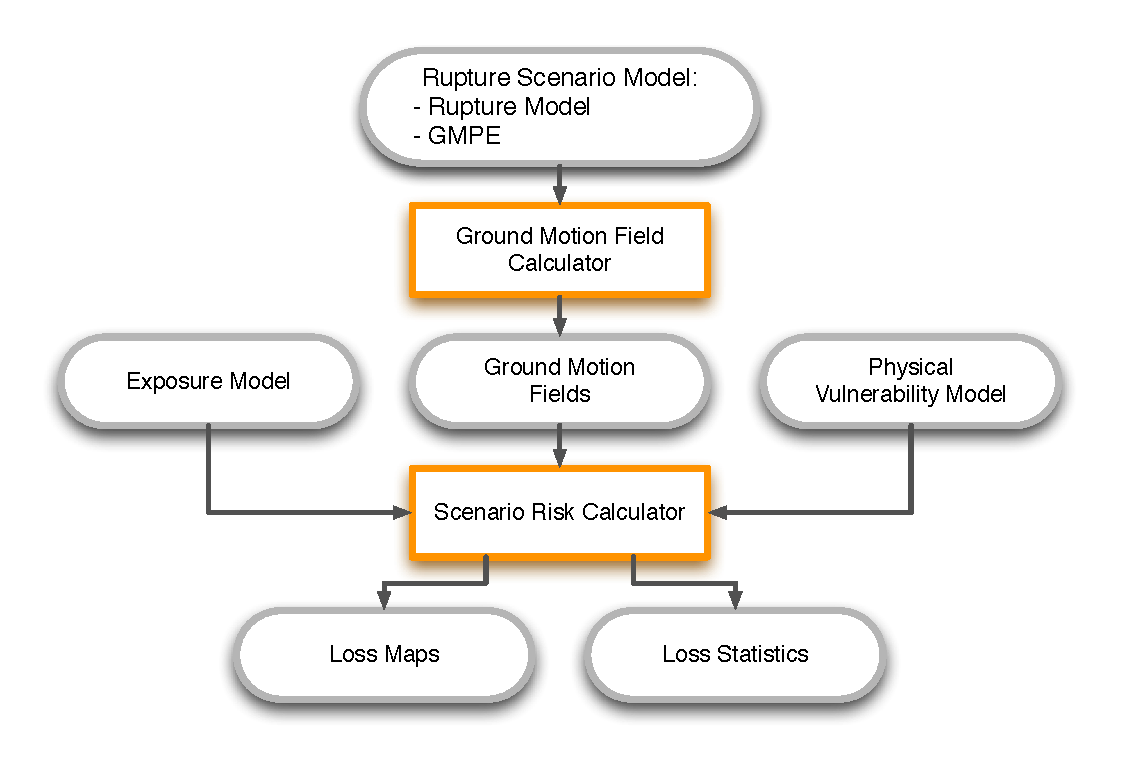
\includegraphics[width=10cm,height=8cm]{./figures/Scheme_Scenario_calc.eps}
\caption{Workflow of the scenario risk calculations.}
\label{fig:Scheme_scenrisk_calc}
\end{figure}
%
For each ground motion field, the intensity measure level at a given 
site is combined with a vulnerability function, from which a loss ratio is randomly sampled, for each asset contained in the exposure model. The loss ratios that are sampled for assets of a given taxonomy classification at different locations are considered to be either independent or fully correlated, knowing that the reality is likely to lie somewhere in between these two assumptions. Using these results, the mean and standard deviation of the loss ratios across all ground motion fields can be calculated. Loss ratios are converted into losses by multiplying by the value of the asset given in the exposure model. It is furthermore possible to sum the losses throughout the region and to compute the mean and standard deviation of the total loss. 

\subsection{Calculation Steps}

To compute the mean loss:

\begin{enumerate}
\item For each ground motion field, the intensity measure level at the location of the asset is used to derive the mean loss ratio and associated coefficient of variation from the vulnerability function. Since currently the vulnerability functions are being defined in a discrete manner, it is quite probable that the intensity measure level provided by the ground motion field is not contained in the vulnerability function. In these cases, linear interpolation methods are being employed to derive the mean loss ratio at the intensity measure level of interest. 

\item The engine takes the vulnerability function assigned to each asset and checks if the coefficient of variation is zero. If so, the loss ratios are derived based on the mean loss ratio for each intensity measure level. Otherwise, if the uncertainty is defined, it is randomly sampled following the probabilistic distribution of the respective vulnerability function, as described below:

\begin{equation}
\log{LR_n} = \mu + \epsilon\sigma
\end{equation}

Where $\mu$ and $\sigma$ stand for the mean and standard deviation of the logarithm of the loss ratios respectively and $\epsilon$ is a term that has a standard normal distribution with a zero mean and a standard deviation of one.  

The method used to sample epsilon can follow two approaches depending on whether the correlation between the vulnerability of assets of a given taxonomy is to be considered or not:

\begin{itemize}

\item Perfectly correlated: the term $\epsilon$ is randomly sampled once for the first asset and this result is used to derive the loss ratio for all the assets of the same taxonomy. 

\item Uncorrelated: the term $\epsilon$ is always randomly sampled for each asset and therefore the correlation between the vulnerability of the assets is ignored.

\end{itemize}

It is expected that the true level of correlation lies somewhere between these two assumptions, and thus they provide boundaries to the expected output. 


\item The mean loss ratio for each asset across all possible simulations of the deterministic event can be calculated through the formula:

\begin{equation}
LR=\frac{\sum^m_{n=1}LR_n|IML}{m}
\end{equation}

Where $m$ stands for the number of ground motion fields simulated.

\item The mean loss can then be derived by multiplying the mean loss ratio by the value of the asset contained in the exposure model file.

\end{enumerate}

To compute the standard deviation of the loss:

\begin{enumerate}

\item In order to compute the uncertainty, the engine takes the set of 
    loss ratios for each asset, and computes the associated standard 
    deviation using the classical formula:

\begin{equation}
SD[LR]=\sqrt{  \frac{1}{m}\sum_{n=1}^m{(LR_n-E[LR])^2} }
\end{equation}

Where $E[LR]$ stands for the mean loss ratio computed previously.

\item The standard deviation of the absolute loss can finally be computed
    by multiplying the standard deviation of the loss ratio by the value 
    of the respective asset.

\end{enumerate}

\subsection{Calculator Output}
The output of the Scenario Risk Calculator currently comprises loss statistics (mean total loss and standard deviation of total loss) and loss maps. Loss maps are comprised by a set of Òloss nodesÓ, which are associated with a pair of coordinates. For each node, one or more loss values might exist, due to the fact that several different assets can be located at the same location.  Figure \ref{fig:detlosses} presents an example of a loss map containing the expected economic losses for reinforced concrete buildings located in the metropolitan area of Istanbul, considering a rupture of magnitude 7.5Mw under the Sea of Marmara.
\begin{figure}[ht]
\centering
\includegraphics[width=12cm,height=9cm]{./figures/LossesDetIstanbul.eps}
\caption{Loss map with the distribution of mean economic losses for reinforced concrete buildings.}
\label{fig:detlosses}
\end{figure} 

\section{Exposure model definition}
All risk calculators in OpenQuake require an exposure model that needs to be stored in NRML. Common to all of the assets stored in a given exposure model, the following metadata needs to be provided, as described below: 

\begin{itemize}
\item  \Verb+id+: a unique key used to identify the exposure model within OpenQuake;
\item  \Verb+assetCategory+: a string used to define the type of assets being stored (e.g: buildings, population);
\item  \Verb+areaType+: flag defining the way this parameter is being provided, as explained later in this section; 
\item  \Verb+areaUnits+: attribute defining the units used to measure the area; 
\item  \Verb+stcoType+: flag defining the way this parameter is being provided, as explained later in this section; 
\item  \Verb+stcoUnits+: attribute defining the units used to measure the structural cost;
\item  \Verb+description+: brief string with further information about the exposure model;
\item  \Verb+taxonomySource+: attribute used to define the taxonomy system being used to classify the assets;
\end{itemize}

The way the information about the characteristics of the assets in an exposure model are  stored can vary strongly depending on the authority in charge of compiling the data. As an example, if national census information is used to estimated the distribution of assets in a given region, it is likely that the number of buildings per unit of area will be used to define the dataset. In the other hand, if simplified methodologies based on population distribution are used for this purpose, then it is likely that the built up area or economic value of each building typology will be used. Thus, the following set of attributes were included in the latest version of the schema for the exposure model:

\begin{itemize}
\item  \Verb+number+: number of assets for a given location;
\item  \Verb+area+: area of the asset typology;
\item  \Verb+stco+: structural cost of the asset (e.g: replacement cost). 
\end{itemize}

While the attribute \Verb+number+ might be a rather simple parameter, the other two can be considerably ambiguous as different ways to define them might be used. With regards to the attribute \Verb+area+, one can either choose to provide the aggregated built up area of a certain building typology per location or the average built up area for a single unit. Similarly, the \Verb+stco+ can also be defined as the aggregated economic value (replacement cost for all the asset at the given location), the cost of replacing a single unit or even the replacement cost for unit of area. To establish the way these two attributes are being defined within the exposure model, two flags have been introduced in the schema model:  \Verb+areaType+ and \Verb+stcoType+. 

Notice that since the attribute \Verb+number+ always represents the same quantity (number of assets in a given location), no flag providing further information about this attribute was introduced. Further information regarding the parameters that are currently being used to define the exposure elements can be found in the OpenQuake book. In order to clarify this methodology, several examples are presented later in this section.

Finally, a pair of coordinates (longitude and latitude) needs to be provided to define the location of each asset.The way this information is being stored is constantly being modified, as further feedback from users and experts is received. Hence, it is important to understand which version of NRML OpenQuake is using, in order to avoid incompatibility issues. NRML is already in its third version (0.3) and documentation about each release can be found on Github. Several examples of exposure models containing different types of information are presented now. Users will notice that some of the attributes are marked with a "\Verb+gml+" tag, which means that these parameters must follow the Geography Markup Language grammar, developed by the Open Geospatial Consortium.\\

\paragraph{Example 1}
This example is comprised by an exposure model in which the aggregated economic value of each building typology for a set of locations is directly provided.

\begin{Verbatim}[frame=single, commandchars=\\\{\}, samepage=false]
<\textcolor{red}{exposurePortfolio} gml:id="ep">
    <\textcolor{green}{exposureList} gml:id="Italy2012_1" assetCategory="buildings" 
    stcoUnit="EUR" stcoType="aggregated">
    <gml:description>Buildings in Italy</gml:description>
    <taxonomySource>Pavia taxonomy</taxonomySource>
        <\textcolor{blue}{assetDefinition} gml:id="asset1">
            <site>
               <gml:Point srsName="epsg:4326">
               <gml:pos>15.22 38.80</gml:pos>
               </gml:Point>
            </site>
            <taxonomy>URM</taxonomy>
            <stco> 500.000 </stco>
        <\textcolor{blue}{/assetDefinition} 
        ...
        <\textcolor{blue}{assetDefinition} gml:id="asset999">
            <site>
               <gml:Point srsName="epsg:4326">
	      <gml:pos>15.23 38.95</gml:pos>
	      </gml:Point>
	   </site>
	   <taxonomy>RC</taxonomy>
	   <stco> 700.000 </stco>
        <\textcolor{blue}{/assetDefinition}> 
    <\textcolor{green}{/exposureList}>
<\textcolor{red}{/exposurePortfolio}>
\end{Verbatim}

Each asset is uniquely identified by its \Verb+id+, which is used by OpenQuake to relate each asset with the associated results (e.g.: loss curves). Then, a pair of coordinates (latitude and longitude) for a \Verb+site+ is defined. This position (\Verb+pos+) and the associated geographical projection (\Verb+srsName+) need to be provided in the \Verb+Point+ attribute. Each asset must to be classified according to a \Verb+taxonomy+, so that OpenQuake is capable of employing the appropriate vulnerability function in the risk calculations. Finally, the value of the asset is stored in the \Verb+stco+ attribute. In this case, the aggregated economic value for the assets at each location if provided directly, so there is no need of defining other attributes such as \Verb+number+ or \Verb+area+. This mode of representing an exposure model is probably simplest way.\\ 

\section{Vulnerability model definition}
In this section, the NRML schema for the vulnerability model is described in detail. In order to do so, a graphical representation of a vulnerability model (mean loss ratio for a set of intensity measure levels) is illustrated in Figure \ref{fig:vulModel}, and the equivalent NRML file is then presented. Note that although the uncertainty for each loss ratio is not represented in the aforementioned figure, it has been considered in the input NRLM file, by means of a coefficient of variation per loss ratio. This model is composed by two discrete vulnerability functions and uses spectral acceleration for a certain period. 

\begin{figure}[ht]
\centering
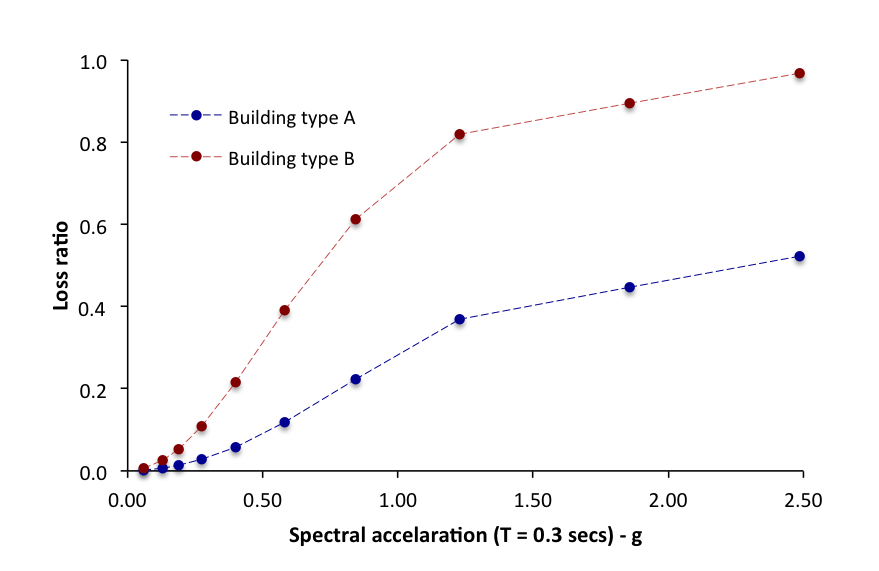
\includegraphics[width=10cm,height=6cm]{./figures/vulnerabilityModel.eps}
\caption{Graphical representation of a vulnerability model.}
\label{fig:vulModel}
\end{figure}

Each component of the associated NRML file is presented herein:

\begin{Verbatim}[frame=single, commandchars=\\\{\}, samepage=true]
<\textcolor{red}{vulnerabilityModel}>
    <\textcolor{green}{discreteVulnerabilitySet} vulnerabilitySetID="OpenQuake2011"	
    assetCategory="buildings"    lossCategory="economic loss">
        ...
\end{Verbatim}

At the top of the NRML schema, the following metadata are being stored:
\begin{itemize}
\item  \Verb+vulnerabilitySetID+: A unique key used to identify the vulnerability model instance within OpenQuake;
\item  \Verb+assetCategory+: An attribute that describes the asset typology (e.g.: population, buildings, contents);
\item  \Verb+lossCategory+: An attribute that describes the type of loss suffered by the assetCategory (e.g.: fatalities, collapse, economic loss). 
\end{itemize}

\begin{Verbatim}[frame=single, commandchars=\\\{\}, samepage=true]
    ...
        <\textcolor{blue}{IML}  IMT = "Sa 0.3"> 0.061 0.129 0.188 0.273 0.398 0.579 
        0.843 1.227 1.856 2.485 <\textcolor{blue}{/IML}>
        ...
\end{Verbatim}

Within this component, an attribute specifying the intensity measure type (e.g.: Sa, PGA, MMI) is defined, followed by the list of intensity measure levels. This set of values is common to all of the vulnerability functions.

\begin{Verbatim}[frame=single, commandchars=\\\{\}, samepage=true]
        ...
        <\textcolor{blue}{discreteVulnerability}  vulnerabilityFunctionID="typeA" 
        probabilisticDistribution="LN">
            <\textcolor{magenta}{meanLossRatio}> 0.002 0.007 0.014 0.028 0.058 0.118
            0.223 0.370 0.446 0.523 <\textcolor{magenta}{/meanLossRatio}>
            <\textcolor{magenta}{coefficientVariation}> 0.012 0.058 0.079 0.159 0.265 
            0.244 0.211 0.152 0.088 0.082 <\textcolor{magenta}{/coefficientVariation}>
        <\textcolor{blue}{/discreteVulnerability}>
        <\textcolor{blue}{discreteVulnerability}  vulnerabilityFunctionID="typeB" 
        probabilisticDistribution="LN">
            <\textcolor{magenta}{meanLossRatio}> 0.006 0.025 0.052 0.108 0.215 0.391	
            0.613 0.820 0.894 0.967 <\textcolor{magenta}{/meanLossRatio}>
            <\textcolor{magenta}{coefficientVariation}> 0.010 0.054 0.082 0.167 0.285 
            0.278 0.261 0.132 0.084 0.021 <\textcolor{magenta}{/coefficientVariation}>
        <\textcolor{blue}{/discreteVulnerability}>
    <\textcolor{green}{/discreteVulnerabilitySet} 
<\textcolor{red}{/vulnerabilityModel}>        
\end{Verbatim}

Finally, for each discrete vulnerability function the following parameters are required:
\begin{itemize}
\item  \Verb+ vulnerabilityFunctionID +: A unique key that is used to relate each vulnerability function with the exposure elements;
\item  \Verb+ probabilisticDistribution +: An attribute that establishes the type of probabilistic distribution followed by the loss ratio uncertainty. At the moment, OpenQuake only supports lognormal distributions, however, other types of distributions such as beta will be incorporated in future releases;
\item  \Verb+ meanLossRatio +: A set of loss ratios (one per each intensity measure level defined previously). These values can represent different losses such as fatality rates (quotient between the number of fatalities and total population exposed) or damage ratio (quotient between the repair cost and the replacement cost of a given structure).
\item  \Verb+ coefficientVariation +: A set of coefficients of variation (one per loss ratio) that describes the uncertainty for different levels of loss. If users do not want to consider the uncertainty, this set of parameters can be set to zero, and OpenQuake assumes each loss ratio as a deterministic value. 
\end{itemize}
